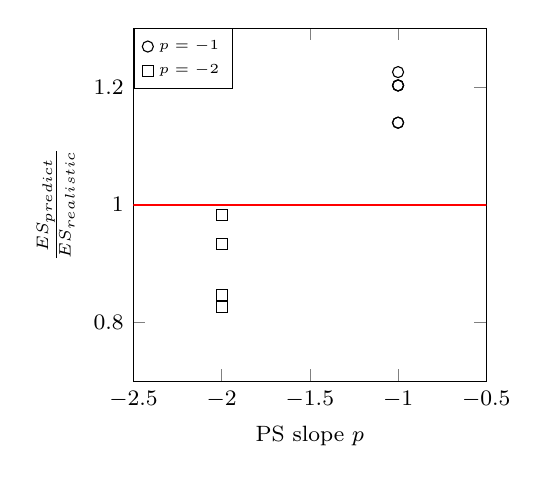
\begin{tikzpicture}[]
        \centering
        \begin{axis}[
            ylabel={$\frac{ES_{predict}}{ES_{realistic}}$},
            xlabel={PS slope $p$},
            ymin=0.7, ymax=1.3,
			xmax=-0.5,
			xmin=-2.5,
			%xtick={-2,-1.5,...,-0.4},
            width=.5\linewidth,
            height=.5\linewidth,
            label style={font=\footnotesize},
			legend style={font=\tiny,at={(0,1)},anchor=north west},
            tick label style={font=\footnotesize}
            ]
			\addplot [
            black,only marks,mark=o,
            ]
            coordinates{
            (-1,1.1394)
            (-1,1.2027)
            (-1,1.2027)
            (-1,1.2254)
            (-1,1.1394)
            (-1,1.2027)
            };
            			\addlegendentry{$p=-1$}
            			\addplot [
            black,only marks,mark=square,
            ]
            coordinates{
            (-2,0.8265)
            (-2,0.9324)
            (-2,0.8456)
            (-2,0.9828)
            (-2,0.8265)
            (-2,0.9324)
            };
            			\addlegendentry{$p=-2$}
			% \fill[color=green!40,opacity=40] (0,1.05) -- (9,1.05) -- (9,0.95) -- (0,0.95) -- cycle;
			 			%\fill[color=yellow!40,opacity=40] (0,0.18) -- (9,9.18) -- (9,8.82) -- (0,-0.18) -- cycle;
						\addplot [
            red,thick,solid,mark=square,
            ]
            coordinates{
            (-3, 1)
            (0, 1)
            };
			%\node[red,right] at (axis cs: 7.8,7.5) {\tiny $\pm5\%$};
        \end{axis}
        \end{tikzpicture}